\documentclass[11pt]{article}

\newcommand{\cnum}{CS M146}
\newcommand{\ced}{Winter 2019}
\newcommand{\ctitle}[3]{\title{\vspace{-0.5in}\cnum, \ced\\Problem Set #1: #2\\Due #3}}
\usepackage{enumitem}
\newcommand{\solution}[1]{{{\color{blue}{\bf Solution:} {#1}}}}
\usepackage[usenames,dvipsnames,svgnames,table,hyperref]{xcolor}
\usepackage{graphicx}
\usepackage[tbtags]{amsmath}
\usepackage[hang, small,labelfont=bf,up]{caption} % Custom captions under/above floats in tables or figures
\usepackage{booktabs} % Horizontal rules in tables


\renewcommand*{\theenumi}{\alph{enumi}}
\renewcommand*\labelenumi{(\theenumi)}
\renewcommand*{\theenumii}{\roman{enumii}}
\renewcommand*\labelenumii{\theenumii.}


\begin{document}
\ctitle{4}{Clustering and PCA}{March 16, 2019}
\author{Tian Ye \\ \small{Collaborator: Derek Chu}}
\maketitle

\newpage

\section{PCA and Image Reconstruction}
\begin{enumerate}
\item 
\solution{
\begin{figure}[!htbp]
    \centering
    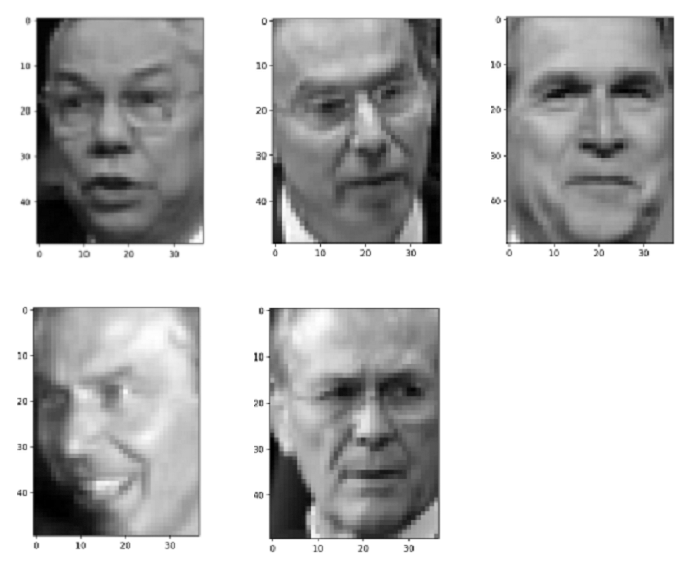
\includegraphics[width=3in]{atotal.png}
    \caption{Example Images} 
\end{figure} \\
\begin{figure}[!htbp]
    \centering
    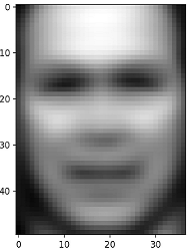
\includegraphics[width=1in]{a6.png}
    \caption{Average Face}
\end{figure} \\
Since the "average face" is the mean of all the other faces, it has no extremely distinct facial feature. Nonetheless, the average still shows signs of general features such as eyes, nose, mouth, etc.
}
\vspace{1cm}
\newpage

\item
\solution{
\begin{figure}[!htbp]
    \centering
    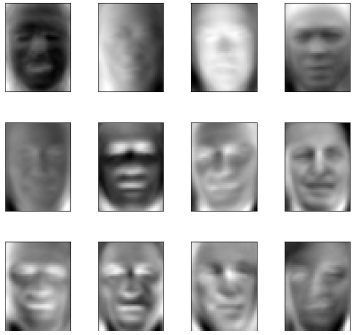
\includegraphics[width=3in]{b.png}
    \caption{Top 12 Eigenfaces} 
\end{figure} \\
These twelve faces were selected as the eigenfaces as these were the ones that exhibited the most prevalent and overarching feature sets of all the faces; they represent a smaller set of base vector images which results in the specific features that arrive.
}

\newpage
\item
\solution{
\begin{figure}[!htbp]
    \centering
    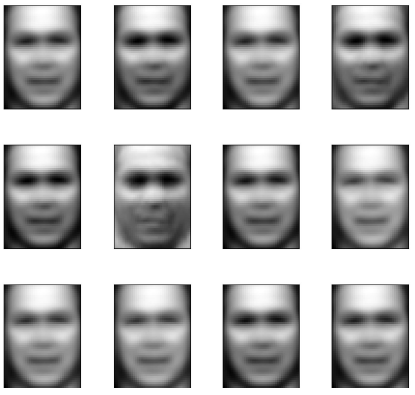
\includegraphics[width=3in]{c1.png}
    \caption{\textit{l} = 1} 
\end{figure} \\
\begin{figure}[!htbp]
    \centering
    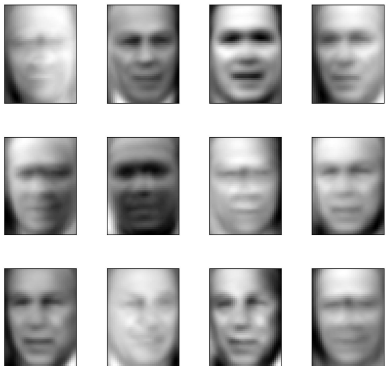
\includegraphics[width=3in]{c10.png}
    \caption{\textit{l} = 10} 
\end{figure} \\
\begin{figure}[!htbp]
    \centering
    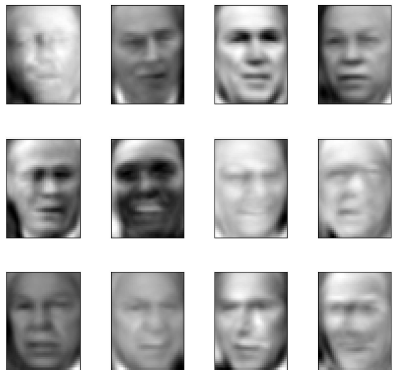
\includegraphics[width=3in]{c50.png}
    \caption{\textit{l} = 50} 
\end{figure} \\
\begin{figure}[!htbp]
    \centering
    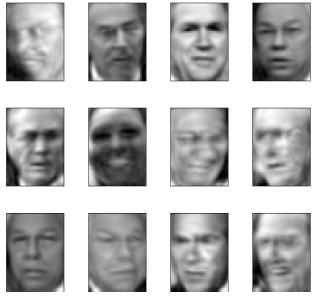
\includegraphics[width=3in]{c100.png}
    \caption{\textit{l} = 100} 
\end{figure} \\
\begin{figure}[!htbp]
    \centering
    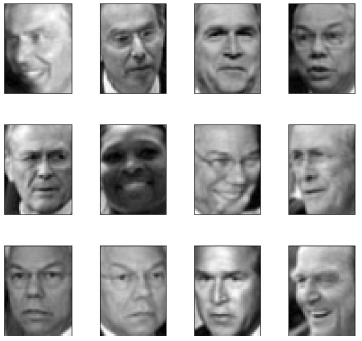
\includegraphics[width=3in]{c500.png}
    \caption{\textit{l} = 500} 
\end{figure} \\
\begin{figure}[!htbp]
    \centering
    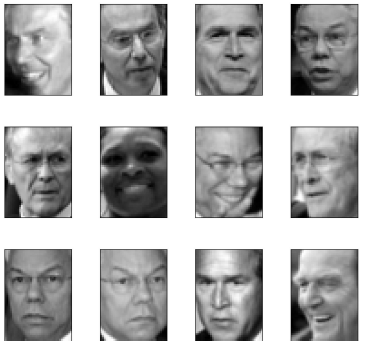
\includegraphics[width=3in]{c1288.png}
    \caption{\textit{l} = 1288} 
\end{figure} \\
As the number of features given to the PCA is increased, so is the facial clarity and feature distinction. This is because as more dimensions are added, more detail is added, hence resulting in improved images.
}
\end{enumerate}
\newpage

\section{\textit{K}-Means and \textit{K}-Medoids}
\begin{enumerate}
\item
\solution{
Attempting to find \textit{k}-clusters while varying $k$ is a bad idea as when $k$ is arbitrary, the algorithm will naturally take the shortest path to minimizing the error to 0. If $k$ is variable, it will increase $k$ until it matches the number of data points; each data point will be its own cluster which will result in 0 error. $k$ would equal $n$, $c$ would equal $i$, and the mean will be the individual coordinates of each individual $x_i$; it would result in overfitting.
}
\item
\solution{Completed.}
\item
\solution{Completed.}
\item
\solution{
\begin{figure}[!htbp]
    \centering
    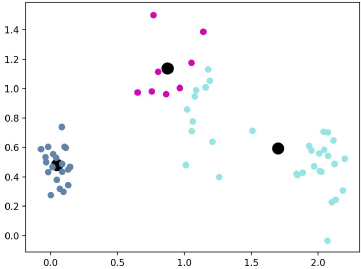
\includegraphics[width=3in]{1randomcentroid.png}
    \caption{Iteration 1 for Random using Centroids} 
\end{figure} \\
\begin{figure}[!htbp]
    \centering
    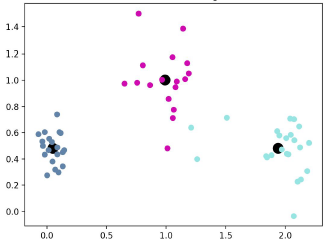
\includegraphics[width=3in]{2randomcentroid.png}
    \caption{Iteration 2 for Random using Centroids} 
\end{figure} \\
\begin{figure}[!htbp]
    \centering
    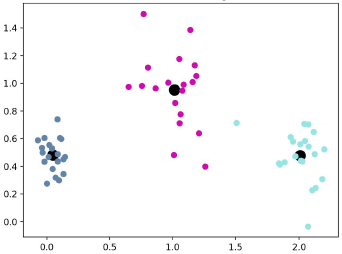
\includegraphics[width=3in]{3randomcentroid.png}
    \caption{Iteration 3 for Random using Centroids} 
\end{figure} \\
\begin{figure}[!htbp]
    \centering
    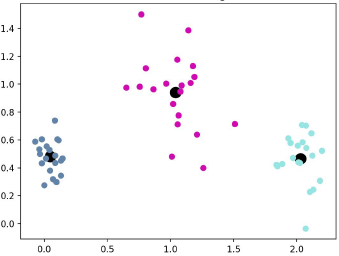
\includegraphics[width=3in]{4randomcentroid.png}
    \caption{Iteration 4 for Random using Centroids} 
\end{figure} \\
\begin{figure}[!htbp]
    \centering
    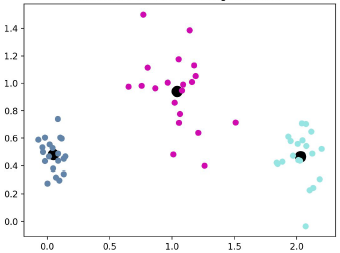
\includegraphics[width=3in]{5randomcentroid.png}
    \caption{Iteration 5 for Random using Centroids} 
\end{figure} \\
}
\newpage
\item
\solution{
\begin{figure}[!htbp]
    \centering
    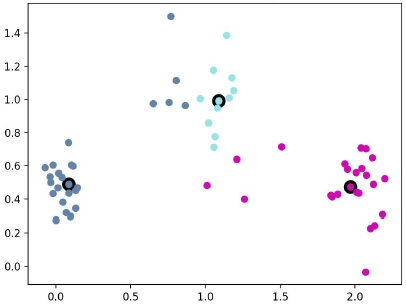
\includegraphics[width=3in]{1randommedoid.png}
    \caption{Iteration 1 for Random using Medoids} 
\end{figure} \\
\begin{figure}[!htbp]
    \centering
    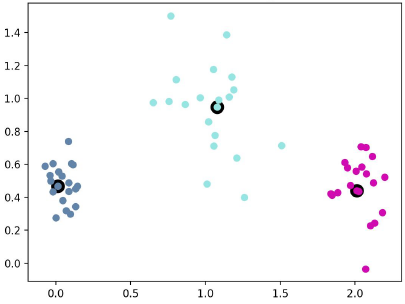
\includegraphics[width=3in]{2randommedoid.png}
    \caption{Iteration 2 for Random using Medoids} 
\end{figure} \\
\begin{figure}[!htbp]
    \centering
    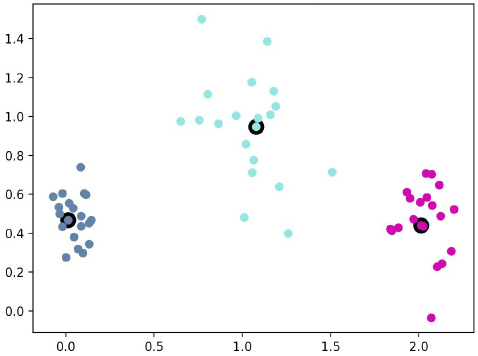
\includegraphics[width=3in]{3randommedoid.png}
    \caption{Iteration 3 for Random using Medoids} 
\end{figure} \\
}
\newpage
\item
\solution{
\begin{figure}[!htbp]
    \centering
    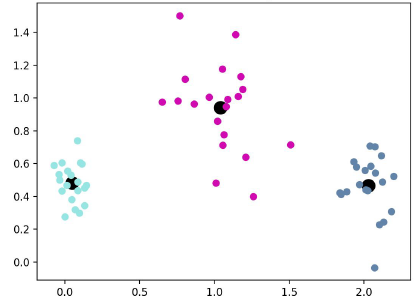
\includegraphics[width=3in]{1cheatcentroid.png}
    \caption{Iteration 1 for Cheat using Centroids} 
\end{figure} \\
\begin{figure}[!htbp]
    \centering
    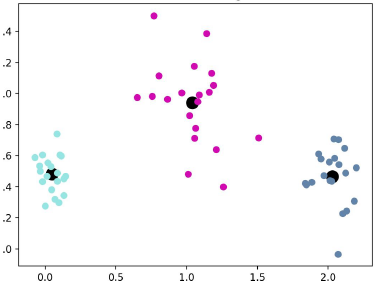
\includegraphics[width=3in]{2cheatcentroid.png}
    \caption{Iteration 2 for Cheat using Centroids} 
\end{figure} \\
}
\newpage
\item
\solution{
\begin{figure}[!htbp]
    \centering
    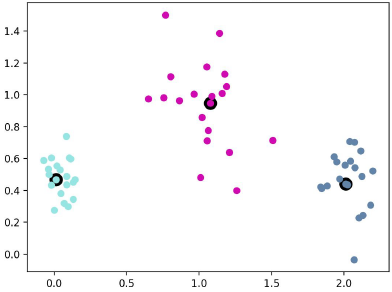
\includegraphics[width=3in]{1cheatmedoid.png}
    \caption{Iteration 1 for Cheat using Medoids} 
\end{figure} \\
\begin{figure}[!htbp]
    \centering
    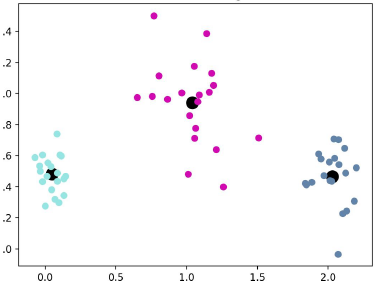
\includegraphics[width=3in]{2cheatcentroid.png}
    \caption{Iteration 2 for Cheat using Medoids} 
\end{figure} \\
}
\end{enumerate}
\newpage

\section{Clustering Faces}
\begin{enumerate}
\item
\solution{
The averages, minimum, and maximum change with seed; however, since we were given a default seed of 1234, that will be the seed we will use. On average, $k$-means has worse performance than $k$-medoids based on pure metric scores; $k$-means does have better efficiency though. $k$-medoids has better performance while having a slower time; this is because $k$-means skew in the presence of outliers while $k$-medoids attempts to achieve a cluster center. Comparing execution times of the two, we see that $k$-means executes faster than $k$-medoids, being {\raise.17ex\hbox{$\scriptstyle\sim$}}0.16 and {\raise.17ex\hbox{$\scriptstyle\sim$}}0.30 respectively.
\begin{table}[!htbp]
\centering
\scalebox{0.8}{
\begin{tabular}{lccc}
\toprule
\cmidrule{1-4}
 & Average & Mininum & Maximum\\
\midrule
$K$-Means & 0.6175 & 0.550 & 0.775 \\
$K$-Medoids &  0.6325 & 0.575 & 0.725 \\
\bottomrule
\end{tabular}}
\end{table} \\
}
\newpage 
\item
\solution{
\begin{figure}[!htbp]
    \centering
    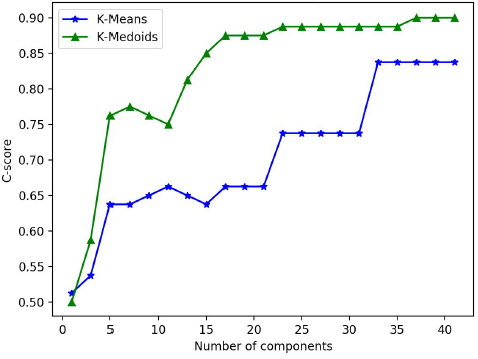
\includegraphics[width=3in]{cscore.png}
    \caption{Cluster Score vs Components} 
\end{figure} \\
Referring to the figure, we can see that the C-score increases proportionally to the number of components for both the $k$-means and $k$-medoid algorithms; this is similar to what we saw in the previous PCA implementations. This is because additionally components permit more feature to manifest, resulting in a higher clustering score.
}

\item
\solution{
For my algorithm, I wrote a design that simply paired two faces and compared them using two clusters and the cheat optimization. It would then run that comparison over all possible combinations of faces and rank all the scores, selecting the lowest and highest scores which represented the easist and hardest faces to cluster, respectively. The faces that were ultimately selected were 4 and 5 with a score of 0.5125 as well as 9 and 16 with a score of 0.9875. Faces 4 and 5 have similar mouths, noses, and eyes as well as having the same skin tone, while 9 and 16 are distinct not only by the shape of the facial features but also by their different skin tones.
\begin{figure}[!htbp]
    \centering
    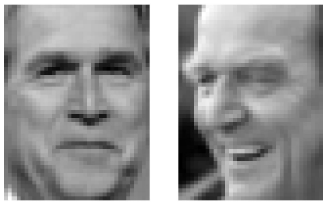
\includegraphics[width=3in]{45.png}
    \caption{Faces 4 and 5} 
\end{figure} \\
\begin{figure}[!htbp]
    \centering
    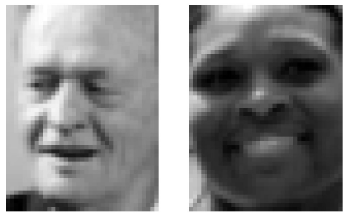
\includegraphics[width=3in]{916.png}
    \caption{Faces 9 and 16} 
\end{figure} \\
}
\end{enumerate}
\end{document}